\documentclass{beamer}
\usepackage[utf8]{inputenc}
\usepackage[francais]{babel}
\usepackage[utf8]{inputenc}  
\usepackage{listings}
\usepackage{graphicx}
\usepackage{color}
\usepackage{float}
\usepackage{algorithm}
\usepackage{algorithmic}
\usepackage{caption}

\usepackage{array}
\usepackage{colortbl}
\usepackage{amsfonts}
\usepackage{geometry}
\usepackage{setspace}
\usepackage{hyperref}
\usepackage{subcaption}
\usepackage{listings}
\usetheme{Warsaw}
\setbeamertemplate{footline}[frame number]

\PassOptionsToPackage{demo}{graphicx}




\author{Adrien Guilbaud}
\title{Simulation numérique directe de la combustion turbulente}
%\subtitle{Presentation Subtile}
%\institute{Université de Bordeaux}
%\date{\today}


%\titlegraphic{
\includegraphics[width=2cm]{figures/logo_fac.jpg}\hspace*{4.75cm}~%
%   
\includegraphics[width=2cm]{figures/logo_cerfacs.eps}
%}

\def\mathunderline#1#2{\color{#1}\underline{{#2}}\color{black}}

\begin{document}
 \AtBeginSection[]
{
  \begin{frame}
    %\frametitle{Table of Contents}
    \tableofcontents[currentsection]
	\addtocounter{framenumber}{-1}

  \end{frame}
}

\begin{frame}[plain]
    \parbox[c]{-50cm}{\centering%
      
\includegraphics[width=2cm]{figures/logo_fac.jpg}%
    }%
    \parbox[c]{19.5cm}{\centering%
      
\includegraphics[width=2cm]{figures/logo_cerfacs.eps}
    }%
\maketitle

\centering
\footnotesize
\begin{tabular}{cc}
  Maître de stage & Enseignant responsable \\
  Mme.~Isabelle \textsc{D'ast} &   M.~Samuel \textsc{Thibault} \\
\end{tabular}
\end{frame}

%
% INTRO
%

\section{Introduction}
\subsection{Présentation du Cerfacs}
\begin{frame}
  \begin{itemize}
  \item Centre de recherche en calcul scientifique
  \item Actionnaires: Airbus Group, Cnes, EDF, Météo France, Onera, Safran et Total
    
  \item Résolution de problèmes scientifiques par la résolution numérique liés :
    \begin{itemize}
    \item au climat
    \item à l'aéronautique
    \item au spatial
    \item à l'environnement
    \end{itemize}
  \item Équipe CSG + équipe CFD
  \end{itemize}
\end{frame}



%https://en.wikipedia.org/wiki/Discretization_of_Navier%E2%80%93Stokes_equations
\subsection{Mécanique des fluides numérique}
\begin{frame}
  \begin{block}{Mécanique des fluides}
    Étude du comportement des fluides lorsqu'ils sont en mouvement
  \end{block}
  
  \begin{itemize}
  \item Résolution d'équations aux dérivées partielles
    \begin{itemize}
    \item Fluides parfaits: Euler
    \item Fluides newtoniens: Navier-Stokes (prix du millénaire)
    \end{itemize}
  \item Mécanique des fluides numérique $\Rightarrow$ discrétisation de l'espace
  \end{itemize}

  \centering
  \visible<2->{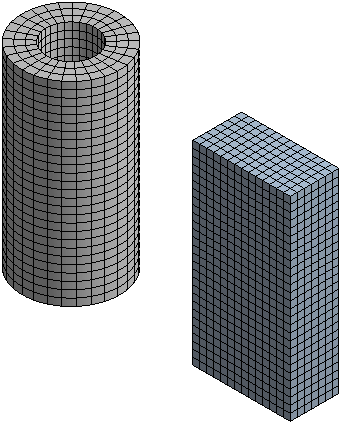
\includegraphics[scale=0.25]{regular-mesh.png}}
  %\visible<2->{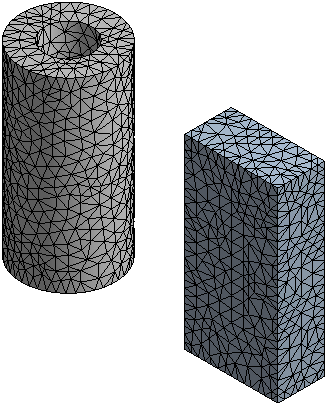
\includegraphics[scale=0.25]{irregular-mesh.png}}
  
\end{frame}


\subsection{Simulation de la turbulence}
\begin{frame}
  Écoulement turbulent $\Rightarrow$ apparition de tourbillons instables
  \begin{itemize}
  \item \textit{DNS}: Direct Numerical Simulation
  \item \textit{LES}: Large Eddy Simulation
  \end{itemize}

  \begin{figure}[ht]
    \centering
    \begin{subfigure}[b]{0.5\textwidth}
      \centering
      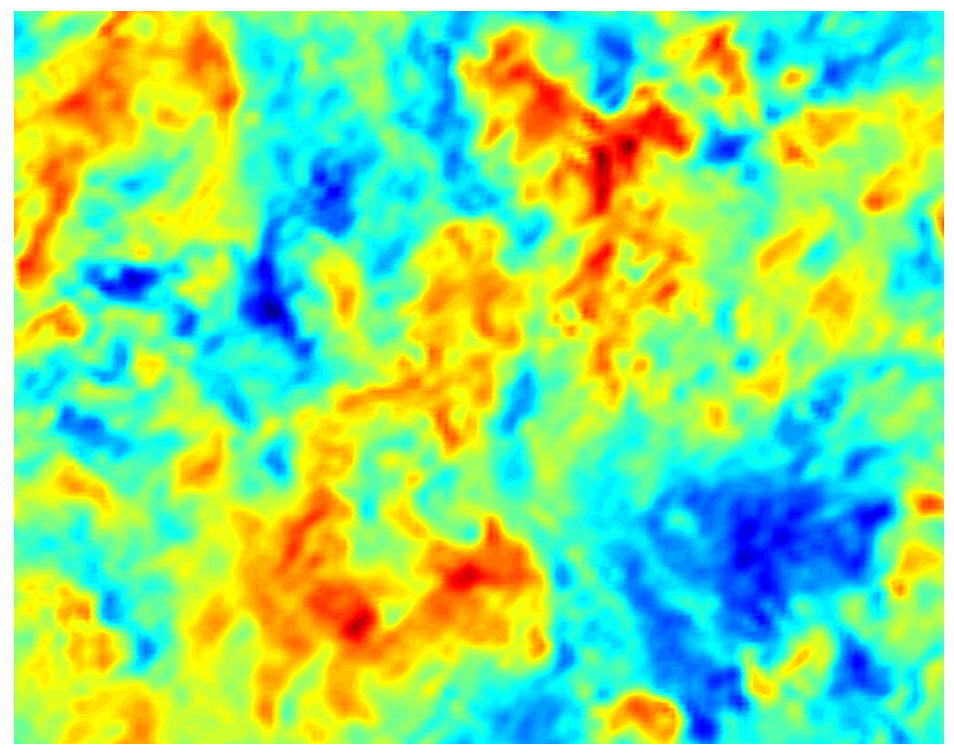
\includegraphics[scale=0.25]{figures/DNS_Velocity_Field.png}
      \caption{\label{fig:dns} DNS}
    \end{subfigure}%
    ~
    \begin{subfigure}[b]{0.5\textwidth}
      \centering
      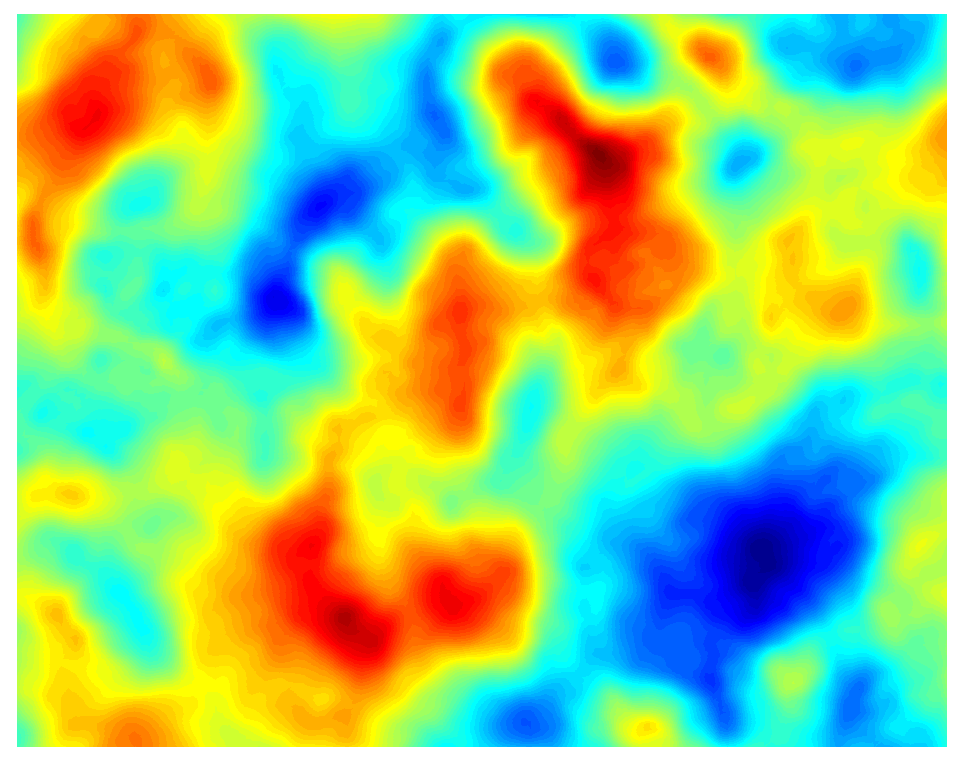
\includegraphics[scale=0.25]{figures/DNS_Filtered_Velocity_Field_Large.png}
      \caption{\label{fig:les} LES}
    \end{subfigure}
  \end{figure}
\end{frame}




%
% Présentation stage
%
\section{Présentation du stage}
\subsection{NTMIX\_CHEMKIN}
\begin{frame}
  \textit{NTMIX\_CHEMKIN}: solveur implicite d'écoulements réactifs
  \begin{itemize}
  \item bidimensionnel
  \item approche DNS
  \item résolution des équation de Navier-Stokes
  \item maillage structuré
  \item discrétisation temporelle (Runge-Kutta)
  \end{itemize}
  
  \vfill
  Utilité:
  \begin{itemize}
  \item Intérêt en recherche fondamentale
  \item Permet de développer des modèles de turbulence
  \end{itemize}
\end{frame}


\subsection{Objectifs}
\begin{frame}

  \begin{block}{Objectif}
    Développer une version 3D et parallèle de \textit{NTMIX}
  \end{block}
  \begin{itemize}
  \item Modernisation du code
  \item Développement de la version tridimensionnelle
  \item Parallélisation la version 3D
  \item Étude des performances
  \end{itemize} 
\end{frame}


%
% Parallélisation
%

\section{Parallélisation de NTMIX}
\subsection{Décomposition de domaine}
\begin{frame}
  \begin{block}{Objectif}
    Exécuter NTMIX sur de grands maillages ($\approx 10^9$ points)
  \end{block}
  \pause
  \begin{alertblock}{Limitations matérielles}
    \begin{itemize}
    \item     Mémoire globale nécessaire: 
      $$10^9pts \times (5+300) \times 8o \approx 2.2 \text{ To}$$
    \item     Temps de calcul: 
      $$10^9 pts\times(4\times10^{-6})s/p\times10000it\approx463 \text{ jours}$$
    \end{itemize}
  \end{alertblock}
  
\end{frame}


\begin{frame}
  \begin{itemize}
  \item Décomposition du domaine
    \begin{itemize}
    \item Division de la mémoire 
    \item Division de la charge de calcul
    \end{itemize}
  \item MPI (\textit{Message Passing Interface})
  \item Topologie cartésienne 
  \end{itemize}

  \centering
  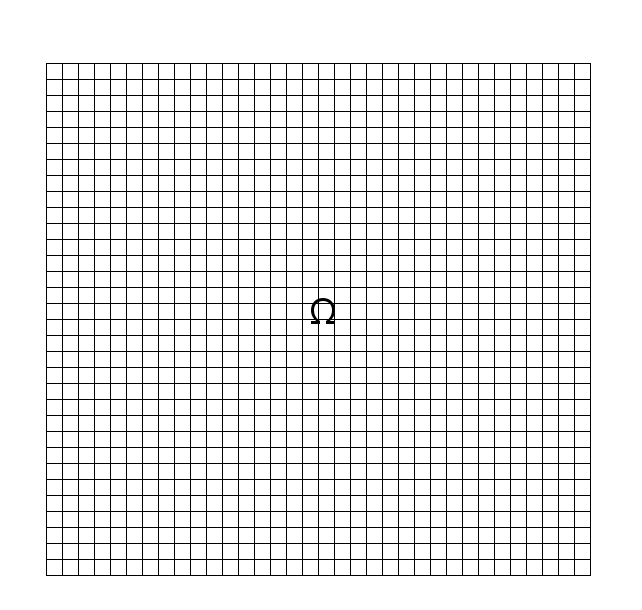
\includegraphics[scale=0.15]{slide_decompo_1.png}$\Rightarrow$
  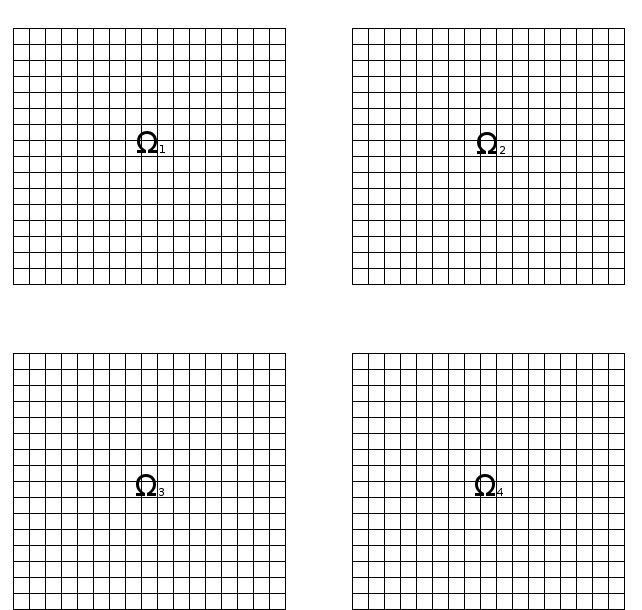
\includegraphics[scale=0.15]{slide_decompo_2.png}
\end{frame}



\begin{frame}
  \begin{alertblock}{Problème}
    Des points manquent d'informations pour le calcul des dérivées
  \end{alertblock}

  \footnotesize

  %\only<2>{$$3\bigg( \frac{\partial u}{\partial x}\bigg) _{i-1} + 9\mathunderline{green}{\bigg( \frac{\partial u}{\partial x}\bigg) _{i}} + 3\bigg( \frac{\partial u}{\partial x}\bigg) _{i+1} = \frac{1}{h}\left(  \frac{1}{4} ( u_{i+2}-u_{i-2} ) + 7 ( u_{i+1} - u_{i-1} ) \right) $$}


  %\only<3>{$$3\bigg( \frac{\partial u}{\partial x}\bigg) _{i-1} + 9\mathunderline{green}{\bigg( \frac{\partial u}{\partial x}\bigg) _{i}} + 3\bigg( \frac{\partial u}{\partial x}\bigg) _{i+1} = \frac{1}{h}\left(  \frac{1}{4} ( \mathunderline{red}{ u_{i+2}}-\mathunderline{red}{u_{i-2}} ) + 7 ( \mathunderline{red}{u_{i+1}} - \mathunderline{red}{u_{i-1}} ) \right) $$}

  \visible<2->{$$3\only<4->{\mathunderline{red}}{\bigg( \frac{\partial u}{\partial x}\bigg) _{i-1}} + 9\only<2->{\mathunderline{blue}}{\bigg( \frac{\partial u}{\partial x}\bigg) _{i}} + 3\only<4->{\mathunderline{red}}{\bigg( \frac{\partial u}{\partial x}\bigg) _{i+1}} = \frac{1}{h}\left(  \frac{1}{4} ( \only<3->{\mathunderline{red}}{ u_{i+2}}-\only<3->{\mathunderline{red}}{u_{i-2}} ) + 7 ( \only<3->{\mathunderline{red}}{u_{i+1}} - \only<3->{\mathunderline{red}}{u_{i-1}} ) \right) $$}

  \renewcommand{\arraystretch}{1.2}

  \centering
  \visible<2->{
    \begin{tabular}{|c|c|c|c|c|c|c|c|c|}
      \hline
      ... & $u_{i-3}$ & \only<3->{\cellcolor{red!70}}$u_{i-2}$ & \only<3->{\cellcolor{red!70}} $u_{i-1}$ & $u_{i}$ & \only<3->{\cellcolor{red!70}}$u_{i+1}$ & \only<3->{\cellcolor{red!70}}$u_{i+2}$ & $u_{i+3}$ & ... \\
      \hline
      ... & $\frac{\partial u}{\partial x}_{i-3}$ & $\frac{\partial u}{\partial x}_{i-2}$ & $\only<4->{\cellcolor{red!70}}\frac{\partial u}{\partial x}_{i-1}$ & \cellcolor{blue!70} $\frac{\partial u}{\partial x}_{i}$ & $\only<4->{\cellcolor{red!70}}\frac{\partial u}{\partial x}_{i+1}$ & $\frac{\partial u}{\partial x}_{i+2}$ & $\frac{\partial u}{\partial x}_{i+3}$  & ... \\
      \hline
  \end{tabular}}

\end{frame}

\begin{frame}
  \frametitle{Recouvrement de domaines}
  \centering
  \only<1>{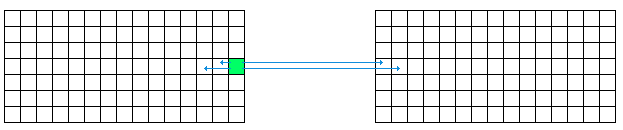
\includegraphics[scale=0.5]{slide_overlap_1.png}\\}
  \only<2->{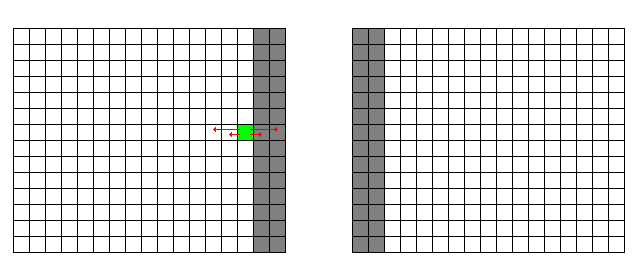
\includegraphics[scale=0.5]{slide_overlap_2.png}}

  \visible<3>{\begin{itemize}
  \item La taille du recouvrement dépend de l'ordre du schéma 
  \item \textit{NTMIX} $\Rightarrow$ schéma d'ordre élevé
  \end{itemize}}
\end{frame}

\begin{frame}
  \frametitle{Traitement des bordures internes}
  \begin{itemize}
  \item   Traitement des bordures des sous-domaines ?
  \item   Utilisation d'un schéma décentré 
  \item   Réduction de l'influence des bordures internes
  \end{itemize}
  \vspace{1cm}
  \centering
  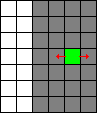
\includegraphics[scale=0.4]{slide_border_1.png}\hspace{2.5cm}
  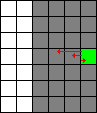
\includegraphics[scale=0.4]{slide_border_2.png}
  %\footnotesize
  %\begin{subequations}
  %\begin{align*}
  %\left( \frac{\partial u}{\partial x}\right) _{i-1} + 4 \left( \frac{\partial u}{\partial x}\right) _{i}  +  \left( \frac{\partial u}{\partial x}\right) _{i-1} &= \frac{1}{h}\left( \frac{1}{3} \left( u_{i+1} - u_{i-1} \right) \right)
  %\end{align*}
  %\end{subequations}
  
\end{frame}

%\begin{frame}
%  Méthode Schwarz:
%  \begin{itemize}
%  \item Couplage inter-domaine élevé
%  \item $\nearrow$ communications
%  \item $\searrow$ taille des communications
%  \end{itemize}
%  Problème local modifié:
%  \begin{itemize}
%  \item Couplage inter-domaine faible
%  \item $\searrow$ communications
%  \item $\nearrow$ taille des communications
%  \end{itemize}
%\end{frame}


%\begin{frame}
%
%  \centering
%    \only<1>{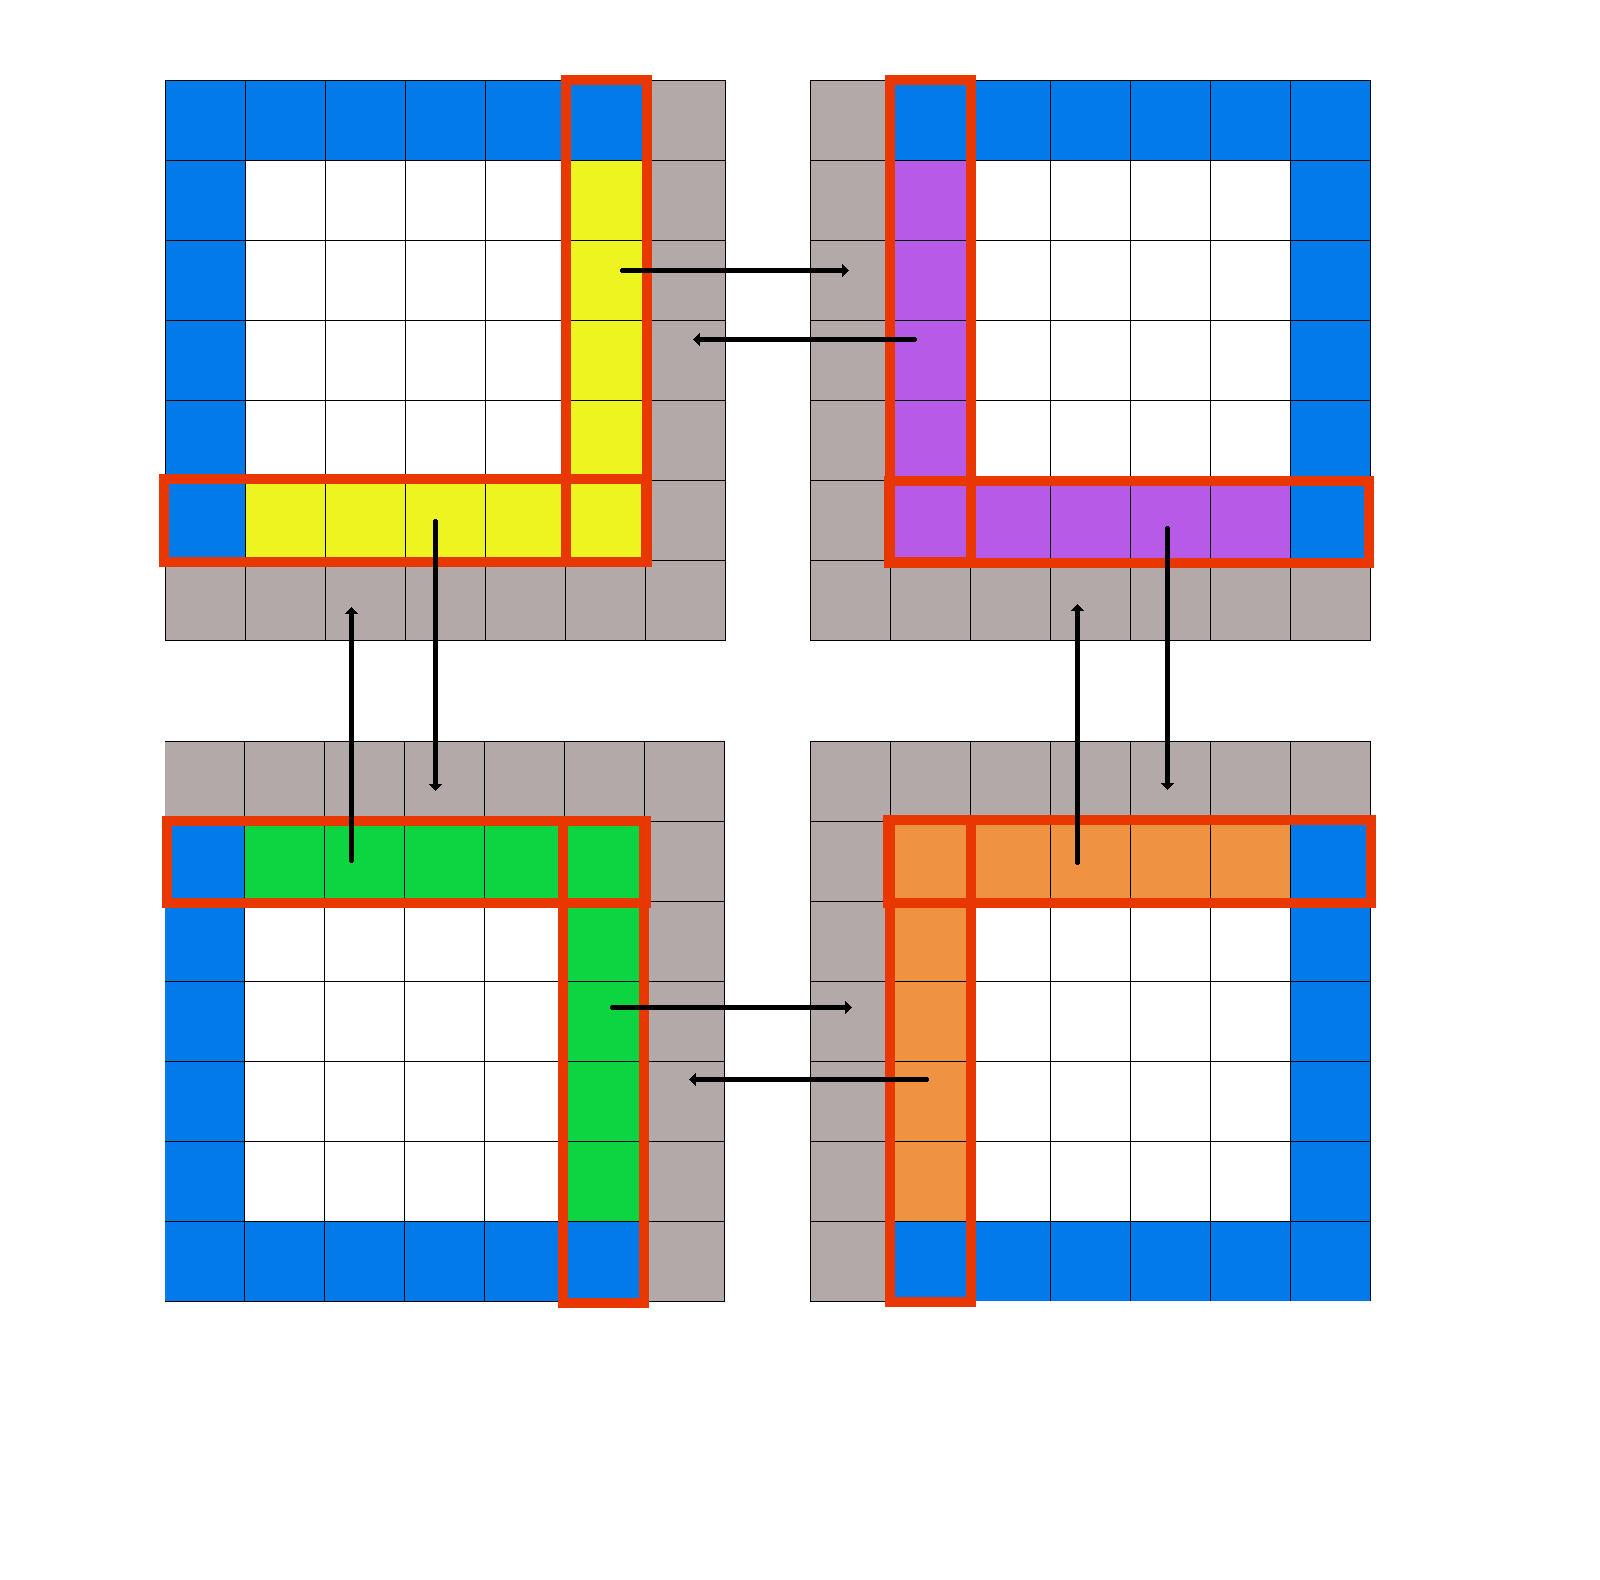
\includegraphics[scale=0.15]{slide_neigh_1.png}\\}
%    \only<2>{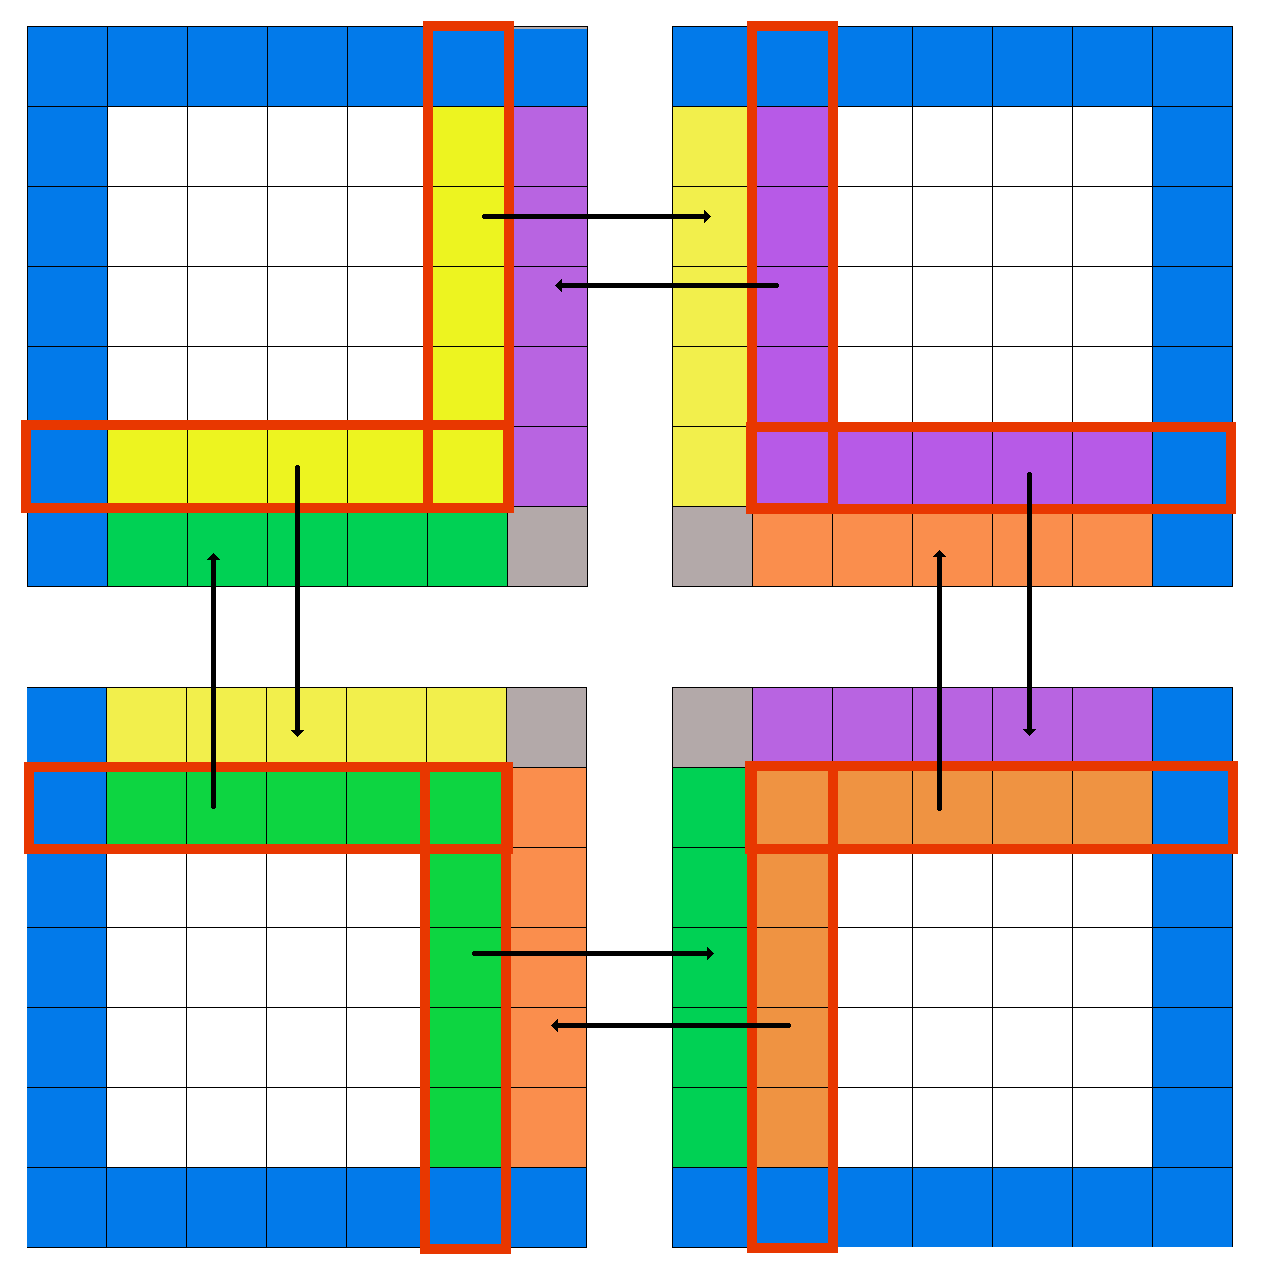
\includegraphics[scale=0.15]{slide_neigh_2.png}\\}
%    \only<3>{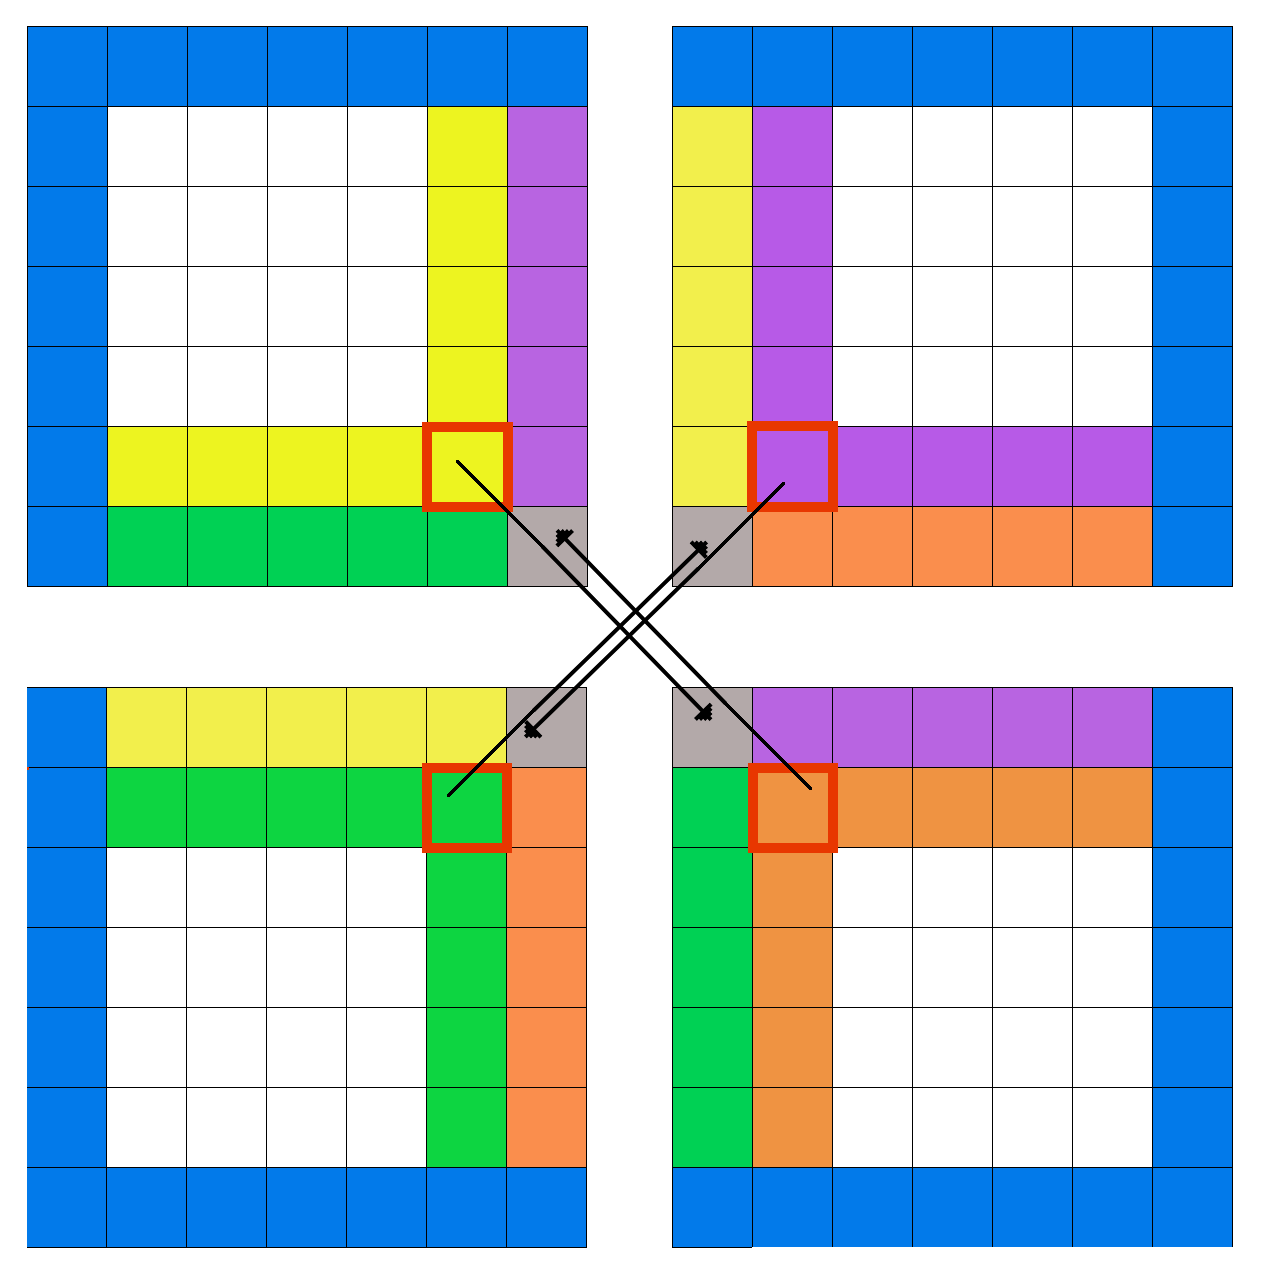
\includegraphics[scale=0.15]{slide_neigh_3.png}\\}
%    \only<4>{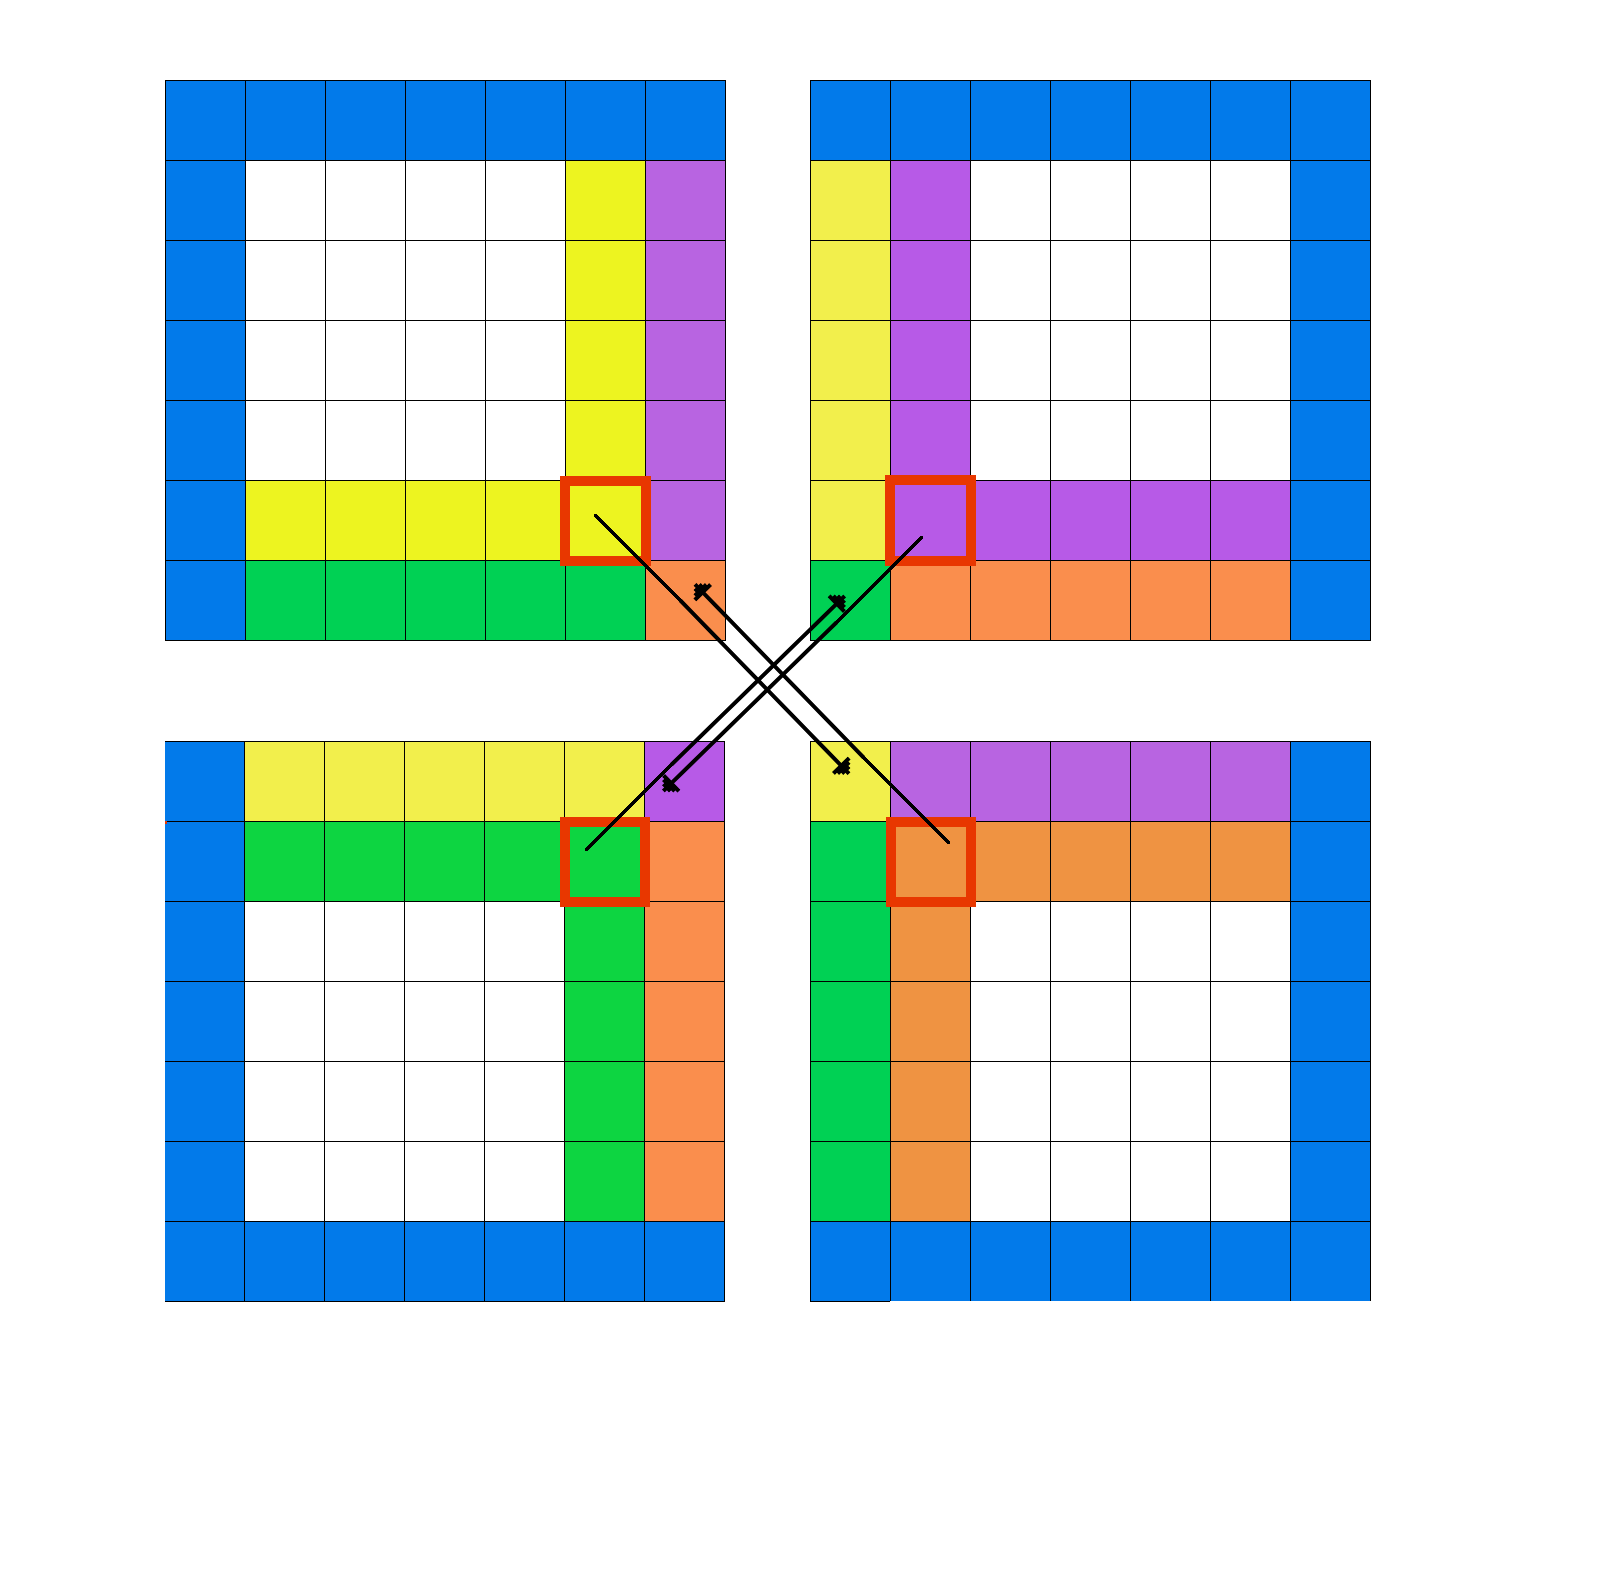
\includegraphics[scale=0.15]{slide_neigh_4.png}}
%\end{frame}

\subsection{Communications}
\begin{frame}
  \frametitle{Échange des points de recouvrement}
  \centering
  \only<1>{Communications sur $x$\\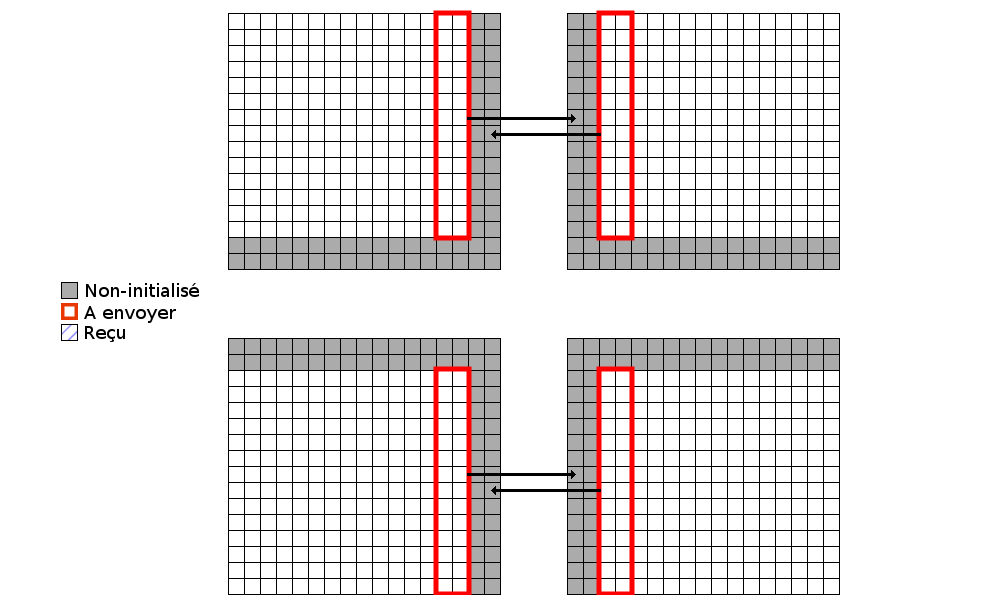
\includegraphics[scale=0.3]{slide_overlapcom_1.png}\\}
  \only<2>{Synchronisation\\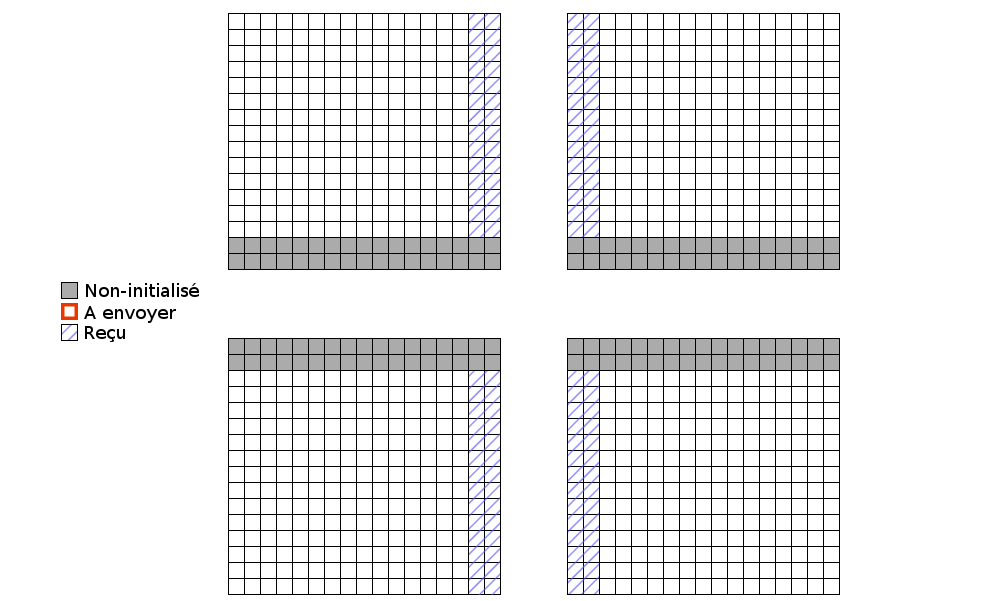
\includegraphics[scale=0.3]{slide_overlapcom_2.png}\\}
  \only<3>{Communications sur $y$\\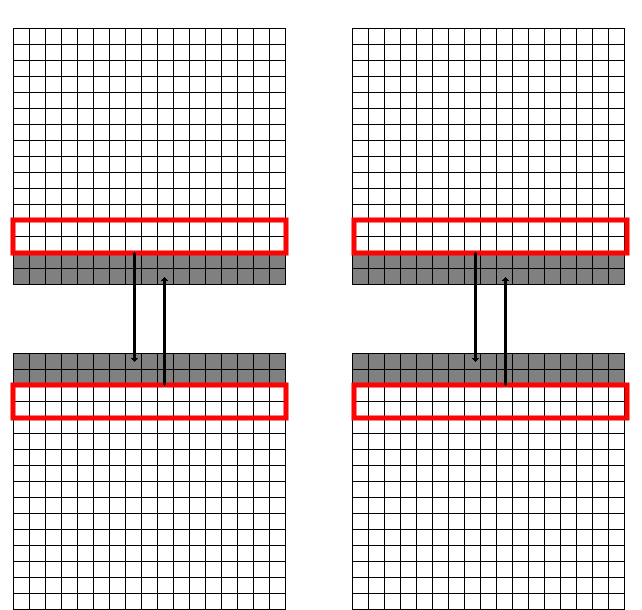
\includegraphics[scale=0.3]{slide_overlapcom_3.png}\\}
  \only<4>{État après les communications\\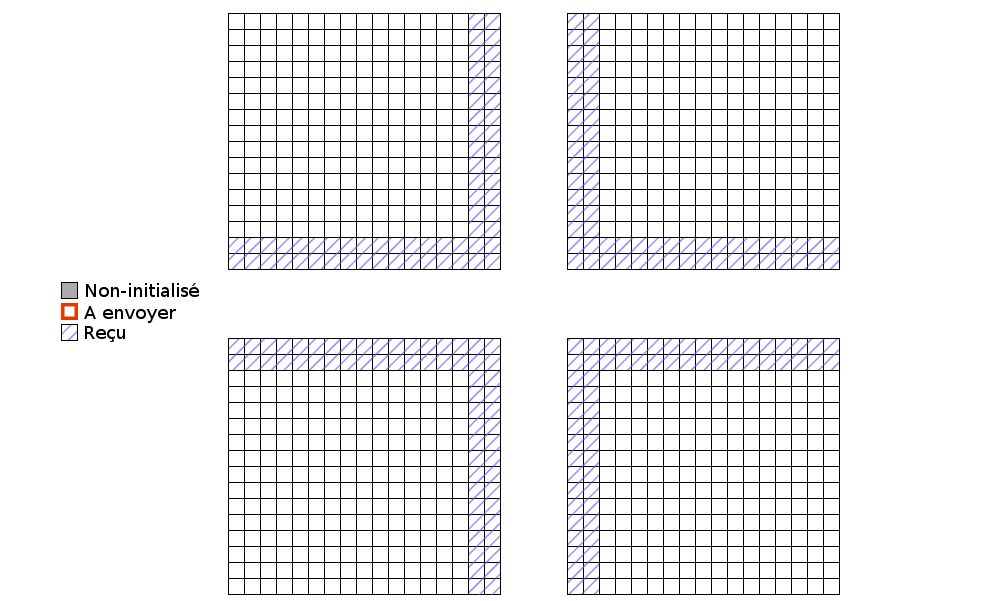
\includegraphics[scale=0.3]{slide_overlapcom_4.png}\\}
\end{frame}


\begin{frame}
  \frametitle{Bilan}
  \begin{itemize}
  \item Schémas moins précis sur les frontières
  \item 1 communication des points de recouvrement/itération de Runge-Kutta
  \item Couplage faible
  \item Duplication du calcul des points de recouvrement
  \end{itemize}
\end{frame}

%
% Performances
%

\section{Etude des performances}
\subsection{Scalabilité forte}
\begin{frame}
  Scalabilité forte:
  \begin{itemize}
  \item domaine global de $400^3$
  \item augmentation progressive du nombre de nœuds
  \end{itemize}
  \vfill
  Speedup: $$S=\frac{t_1}{t_n}$$
\end{frame}


\begin{frame}
  \begin{itemize}
  \item Intel Haswell bi-socket, 12 coeurs 2.5GHz
  \end{itemize}%
  \centering
  \only<1>{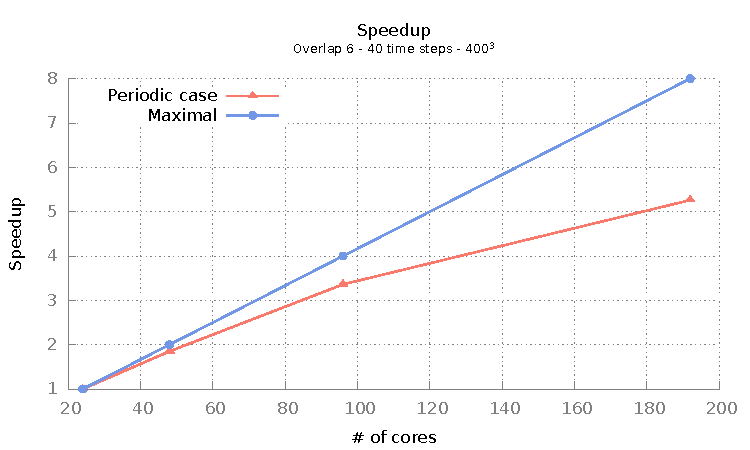
\includegraphics[page=1,scale=0.8]{gnuplot/bench_strong_nemo.pdf}}
  \only<2>{\includegraphics[page=2,scale=0.8]{gnuplot/bench_strong_nemo.pdf}} 
\end{frame}

%
% Conclusion
%
\section{Conclusion}
\begin{frame}
  \begin{itemize}
  \item Version tridimensionnelle de \textit{NTMIX}
  \item Version parallèle
  \item Améliorations encore possibles
    \begin{itemize}
    \item Version hybride OpenMP + MPI
    \end{itemize}
  \end{itemize}

\end{frame}

\begin{frame}
  \centering Merci
  
\end{frame}

\end{document}

